\documentclass[twoside]{book}

% Packages required by doxygen
\usepackage{fixltx2e}
\usepackage{calc}
\usepackage{doxygen}
\usepackage[export]{adjustbox} % also loads graphicx
\usepackage{graphicx}
\usepackage[utf8]{inputenc}
\usepackage{makeidx}
\usepackage{multicol}
\usepackage{multirow}
\PassOptionsToPackage{warn}{textcomp}
\usepackage{textcomp}
\usepackage[nointegrals]{wasysym}
\usepackage[table]{xcolor}

% Font selection
\usepackage[T1]{fontenc}
\usepackage[scaled=.90]{helvet}
\usepackage{courier}
\usepackage{amssymb}
\usepackage{sectsty}
\renewcommand{\familydefault}{\sfdefault}
\allsectionsfont{%
  \fontseries{bc}\selectfont%
  \color{darkgray}%
}
\renewcommand{\DoxyLabelFont}{%
  \fontseries{bc}\selectfont%
  \color{darkgray}%
}
\newcommand{\+}{\discretionary{\mbox{\scriptsize$\hookleftarrow$}}{}{}}

% Page & text layout
\usepackage{geometry}
\geometry{%
  a4paper,%
  top=2.5cm,%
  bottom=2.5cm,%
  left=2.5cm,%
  right=2.5cm%
}
\tolerance=750
\hfuzz=15pt
\hbadness=750
\setlength{\emergencystretch}{15pt}
\setlength{\parindent}{0cm}
\setlength{\parskip}{3ex plus 2ex minus 2ex}
\makeatletter
\renewcommand{\paragraph}{%
  \@startsection{paragraph}{4}{0ex}{-1.0ex}{1.0ex}{%
    \normalfont\normalsize\bfseries\SS@parafont%
  }%
}
\renewcommand{\subparagraph}{%
  \@startsection{subparagraph}{5}{0ex}{-1.0ex}{1.0ex}{%
    \normalfont\normalsize\bfseries\SS@subparafont%
  }%
}
\makeatother

% Headers & footers
\usepackage{fancyhdr}
\pagestyle{fancyplain}
\fancyhead[LE]{\fancyplain{}{\bfseries\thepage}}
\fancyhead[CE]{\fancyplain{}{}}
\fancyhead[RE]{\fancyplain{}{\bfseries\leftmark}}
\fancyhead[LO]{\fancyplain{}{\bfseries\rightmark}}
\fancyhead[CO]{\fancyplain{}{}}
\fancyhead[RO]{\fancyplain{}{\bfseries\thepage}}
\fancyfoot[LE]{\fancyplain{}{}}
\fancyfoot[CE]{\fancyplain{}{}}
\fancyfoot[RE]{\fancyplain{}{\bfseries\scriptsize Generated by Doxygen }}
\fancyfoot[LO]{\fancyplain{}{\bfseries\scriptsize Generated by Doxygen }}
\fancyfoot[CO]{\fancyplain{}{}}
\fancyfoot[RO]{\fancyplain{}{}}
\renewcommand{\footrulewidth}{0.4pt}
\renewcommand{\chaptermark}[1]{%
  \markboth{#1}{}%
}
\renewcommand{\sectionmark}[1]{%
  \markright{\thesection\ #1}%
}

% Indices & bibliography
\usepackage{natbib}
\usepackage[titles]{tocloft}
\setcounter{tocdepth}{3}
\setcounter{secnumdepth}{5}
\makeindex

% Hyperlinks (required, but should be loaded last)
\usepackage{ifpdf}
\ifpdf
  \usepackage[pdftex,pagebackref=true]{hyperref}
\else
  \usepackage[ps2pdf,pagebackref=true]{hyperref}
\fi
\hypersetup{%
  colorlinks=true,%
  linkcolor=blue,%
  citecolor=blue,%
  unicode%
}

% Custom commands
\newcommand{\clearemptydoublepage}{%
  \newpage{\pagestyle{empty}\cleardoublepage}%
}

\usepackage{caption}
\captionsetup{labelsep=space,justification=centering,font={bf},singlelinecheck=off,skip=4pt,position=top}

%===== C O N T E N T S =====

\begin{document}

% Titlepage & ToC
\hypersetup{pageanchor=false,
             bookmarksnumbered=true,
             pdfencoding=unicode
            }
\pagenumbering{alph}
\begin{titlepage}
\vspace*{7cm}
\begin{center}%
{\Large Snake }\\
\vspace*{1cm}
{\large Generated by Doxygen 1.8.13}\\
\end{center}
\end{titlepage}
\clearemptydoublepage
\pagenumbering{roman}
\tableofcontents
\clearemptydoublepage
\pagenumbering{arabic}
\hypersetup{pageanchor=true}

%--- Begin generated contents ---
\chapter{Hierarchical Index}
\section{Class Hierarchy}
This inheritance list is sorted roughly, but not completely, alphabetically\+:\begin{DoxyCompactList}
\item \contentsline{section}{Game\+Font}{\pageref{struct_game_font}}{}
\item \contentsline{section}{Object}{\pageref{class_object}}{}
\begin{DoxyCompactList}
\item \contentsline{section}{Cherry}{\pageref{class_cherry}}{}
\item \contentsline{section}{Hole}{\pageref{class_hole}}{}
\item \contentsline{section}{Player}{\pageref{class_player}}{}
\item \contentsline{section}{Snake\+Body}{\pageref{class_snake_body}}{}
\item \contentsline{section}{Tree}{\pageref{class_tree}}{}
\item \contentsline{section}{Worm}{\pageref{class_worm}}{}
\end{DoxyCompactList}
\item O\+G\+L\+Game\begin{DoxyCompactList}
\item \contentsline{section}{Snake\+Game}{\pageref{class_snake_game}}{}
\end{DoxyCompactList}
\end{DoxyCompactList}

\chapter{Class Index}
\section{Class List}
Here are the classes, structs, unions and interfaces with brief descriptions\+:\begin{DoxyCompactList}
\item\contentsline{section}{\hyperlink{class_cherry}{Cherry} }{\pageref{class_cherry}}{}
\item\contentsline{section}{\hyperlink{struct_game_font}{Game\+Font} }{\pageref{struct_game_font}}{}
\item\contentsline{section}{\hyperlink{class_hole}{Hole} }{\pageref{class_hole}}{}
\item\contentsline{section}{\hyperlink{class_object}{Object} }{\pageref{class_object}}{}
\item\contentsline{section}{\hyperlink{class_player}{Player} }{\pageref{class_player}}{}
\item\contentsline{section}{\hyperlink{class_snake_body}{Snake\+Body} }{\pageref{class_snake_body}}{}
\item\contentsline{section}{\hyperlink{class_snake_game}{Snake\+Game} }{\pageref{class_snake_game}}{}
\item\contentsline{section}{\hyperlink{class_tree}{Tree} }{\pageref{class_tree}}{}
\item\contentsline{section}{\hyperlink{class_worm}{Worm} }{\pageref{class_worm}}{}
\end{DoxyCompactList}

\chapter{File Index}
\section{File List}
Here is a list of all documented files with brief descriptions\+:\begin{DoxyCompactList}
\item\contentsline{section}{Projects/\+Snake/{\bfseries Cherry.\+h} }{\pageref{_cherry_8h}}{}
\item\contentsline{section}{Projects/\+Snake/{\bfseries Hole.\+h} }{\pageref{_hole_8h}}{}
\item\contentsline{section}{Projects/\+Snake/{\bfseries Movement.\+h} }{\pageref{_movement_8h}}{}
\item\contentsline{section}{Projects/\+Snake/{\bfseries Object.\+h} }{\pageref{_object_8h}}{}
\item\contentsline{section}{Projects/\+Snake/{\bfseries Player.\+h} }{\pageref{_player_8h}}{}
\item\contentsline{section}{Projects/\+Snake/{\bfseries Snake\+Body.\+h} }{\pageref{_snake_body_8h}}{}
\item\contentsline{section}{Projects/\+Snake/{\bfseries Tree.\+h} }{\pageref{_tree_8h}}{}
\item\contentsline{section}{Projects/\+Snake/{\bfseries Worm.\+h} }{\pageref{_worm_8h}}{}
\item\contentsline{section}{Source/\hyperlink{_actions_8h}{Actions.\+h} \\*The Actions file define a thread safe game action }{\pageref{_actions_8h}}{}
\item\contentsline{section}{Source/\hyperlink{_constants_8h}{Constants.\+h} \\*Constants that are used throughout the game }{\pageref{_constants_8h}}{}
\item\contentsline{section}{Source/{\bfseries Game.\+h} }{\pageref{_game_8h}}{}
\item\contentsline{section}{Source/{\bfseries Game\+Font.\+h} }{\pageref{_game_font_8h}}{}
\end{DoxyCompactList}

\chapter{Class Documentation}
\hypertarget{class_cherry}{}\section{Cherry Class Reference}
\label{class_cherry}\index{Cherry@{Cherry}}
Inheritance diagram for Cherry\+:\begin{figure}[H]
\begin{center}
\leavevmode
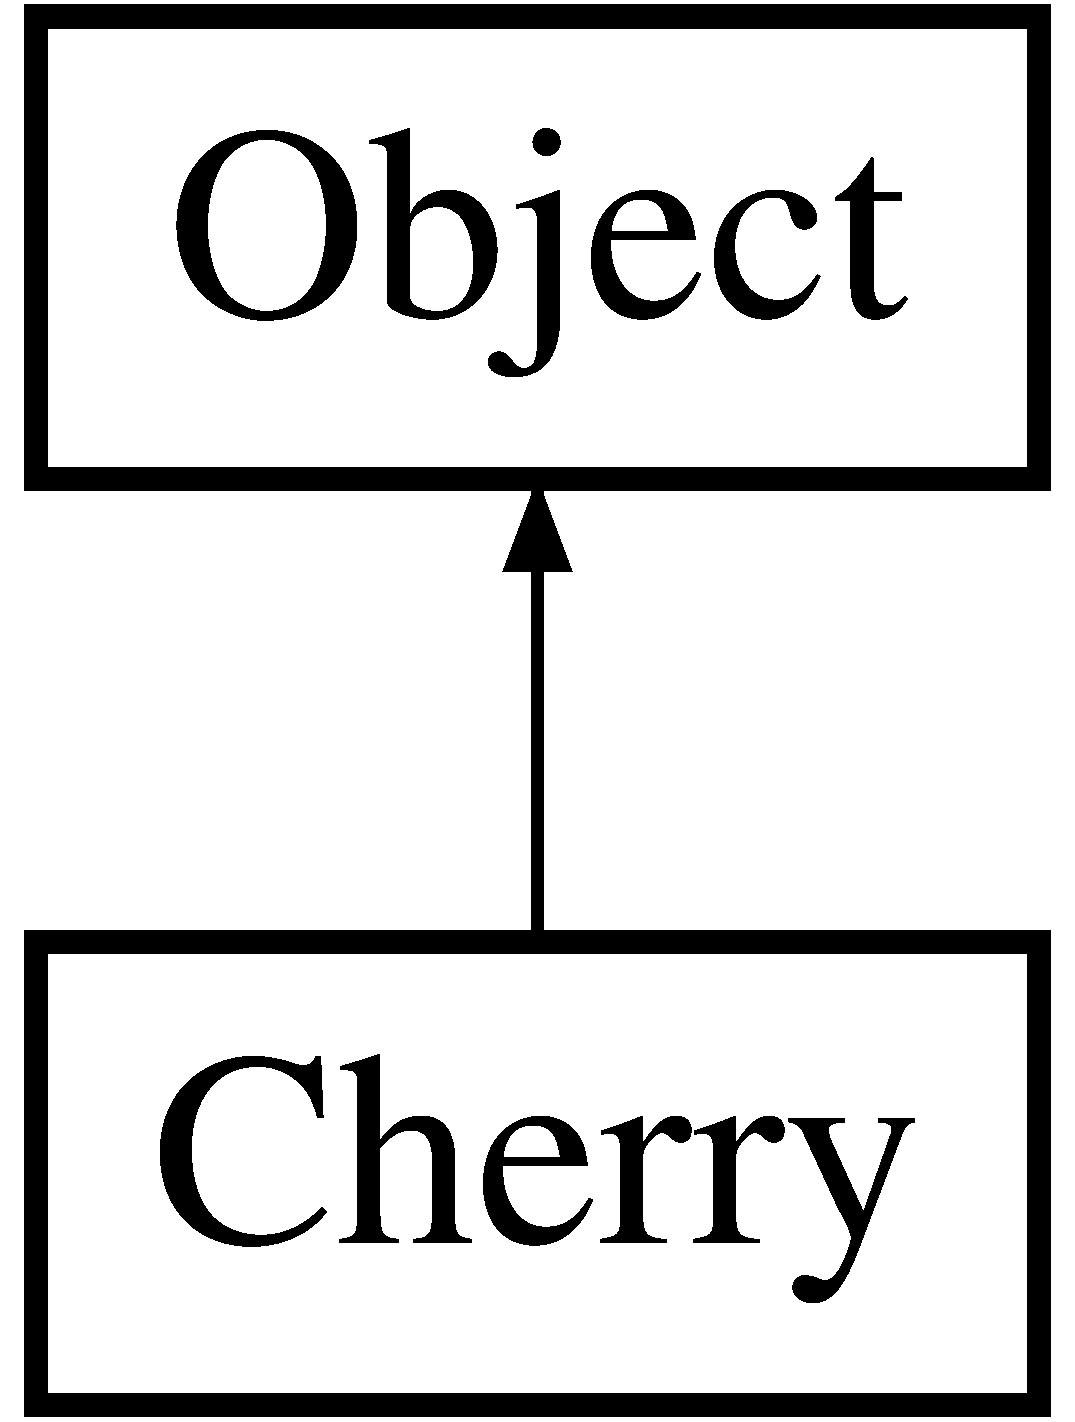
\includegraphics[height=2.000000cm]{class_cherry}
\end{center}
\end{figure}
\subsection*{Public Member Functions}
\begin{DoxyCompactItemize}
\item 
\mbox{\Hypertarget{class_cherry_a7330f4991deb5af8c445e20a0ae2c9f8}\label{class_cherry_a7330f4991deb5af8c445e20a0ae2c9f8}} 
bool {\bfseries load\+Avatar} (A\+S\+G\+E\+::\+Renderer $\ast$renderer)
\item 
\mbox{\Hypertarget{class_cherry_a19bb61762601c45b527a35d9ad0d7f19}\label{class_cherry_a19bb61762601c45b527a35d9ad0d7f19}} 
void {\bfseries set\+PosX} (int x) override
\item 
\mbox{\Hypertarget{class_cherry_a04ee41eb4c488a3f010a44d3d6c545f1}\label{class_cherry_a04ee41eb4c488a3f010a44d3d6c545f1}} 
void {\bfseries set\+PosY} (int y) override
\end{DoxyCompactItemize}
\subsection*{Additional Inherited Members}


The documentation for this class was generated from the following files\+:\begin{DoxyCompactItemize}
\item 
Projects/\+Snake/Cherry.\+h\item 
Projects/\+Snake/Cherry.\+cpp\end{DoxyCompactItemize}

\hypertarget{struct_game_font}{}\section{Game\+Font Struct Reference}
\label{struct_game_font}\index{Game\+Font@{Game\+Font}}


{\ttfamily \#include $<$Game\+Font.\+h$>$}

\subsection*{Public Member Functions}
\begin{DoxyCompactItemize}
\item 
\hyperlink{struct_game_font_af30cf3bbdec633ab3f31491777ad29b6}{Game\+Font} (int idx, char $\ast$n, int ptm)
\begin{DoxyCompactList}\small\item\em Constructor. \end{DoxyCompactList}\end{DoxyCompactItemize}
\subsection*{Public Attributes}
\begin{DoxyCompactItemize}
\item 
int \hyperlink{struct_game_font_ae1e90d4b018bfa8edf42706e245d65f1}{id} = 0
\item 
int \hyperlink{struct_game_font_ae81748d3a1c3b0b53650449e0fd4aeb5}{size} = 0
\item 
char $\ast$ \hyperlink{struct_game_font_a144b59d96bf37c8876b2cd1f7db64d12}{name} = \char`\"{}\char`\"{}
\end{DoxyCompactItemize}
\subsection*{Static Public Attributes}
\begin{DoxyCompactItemize}
\item 
static \hyperlink{struct_game_font}{Game\+Font} $\ast$ \hyperlink{struct_game_font_ac09bfa463d59669ccff031e3e43558ed}{fonts} \mbox{[}5\mbox{]} = \{ nullptr \}
\end{DoxyCompactItemize}


\subsection{Detailed Description}
A loaded font. A font that\textquotesingle{}s loaded in the game engine. 

\subsection{Constructor \& Destructor Documentation}
\mbox{\Hypertarget{struct_game_font_af30cf3bbdec633ab3f31491777ad29b6}\label{struct_game_font_af30cf3bbdec633ab3f31491777ad29b6}} 
\index{Game\+Font@{Game\+Font}!Game\+Font@{Game\+Font}}
\index{Game\+Font@{Game\+Font}!Game\+Font@{Game\+Font}}
\subsubsection{\texorpdfstring{Game\+Font()}{GameFont()}}
{\footnotesize\ttfamily Game\+Font\+::\+Game\+Font (\begin{DoxyParamCaption}\item[{int}]{idx,  }\item[{char $\ast$}]{n,  }\item[{int}]{ptm }\end{DoxyParamCaption})}



Constructor. 

Sets the font index, it\textquotesingle{}s size and description. Make sure the I\+DX is valid otherwise the font will fail to render. 
\begin{DoxyParams}{Parameters}
{\em idx} & is The font index in the Graphics Engine \\
\hline
{\em n} & is the name or description of the font \\
\hline
{\em ptm} & is the size of the loaded font \\
\hline
\end{DoxyParams}
\begin{DoxyReturn}{Returns}
void 
\end{DoxyReturn}


\subsection{Member Data Documentation}
\mbox{\Hypertarget{struct_game_font_ac09bfa463d59669ccff031e3e43558ed}\label{struct_game_font_ac09bfa463d59669ccff031e3e43558ed}} 
\index{Game\+Font@{Game\+Font}!fonts@{fonts}}
\index{fonts@{fonts}!Game\+Font@{Game\+Font}}
\subsubsection{\texorpdfstring{fonts}{fonts}}
{\footnotesize\ttfamily \hyperlink{struct_game_font}{Game\+Font} $\ast$ Game\+Font\+::fonts = \{ nullptr \}\hspace{0.3cm}{\ttfamily [static]}}

Loaded Fonts. Cheap and nasty way of globalising five loaded fonts. \mbox{\Hypertarget{struct_game_font_ae1e90d4b018bfa8edf42706e245d65f1}\label{struct_game_font_ae1e90d4b018bfa8edf42706e245d65f1}} 
\index{Game\+Font@{Game\+Font}!id@{id}}
\index{id@{id}!Game\+Font@{Game\+Font}}
\subsubsection{\texorpdfstring{id}{id}}
{\footnotesize\ttfamily int Game\+Font\+::id = 0}

Font ID. The ID assigned to the font from the graphics engine. \mbox{\Hypertarget{struct_game_font_a144b59d96bf37c8876b2cd1f7db64d12}\label{struct_game_font_a144b59d96bf37c8876b2cd1f7db64d12}} 
\index{Game\+Font@{Game\+Font}!name@{name}}
\index{name@{name}!Game\+Font@{Game\+Font}}
\subsubsection{\texorpdfstring{name}{name}}
{\footnotesize\ttfamily char$\ast$ Game\+Font\+::name = \char`\"{}\char`\"{}}

Name. The name of the font. \mbox{\Hypertarget{struct_game_font_ae81748d3a1c3b0b53650449e0fd4aeb5}\label{struct_game_font_ae81748d3a1c3b0b53650449e0fd4aeb5}} 
\index{Game\+Font@{Game\+Font}!size@{size}}
\index{size@{size}!Game\+Font@{Game\+Font}}
\subsubsection{\texorpdfstring{size}{size}}
{\footnotesize\ttfamily int Game\+Font\+::size = 0}

The font size. The size of the font that was loaded. 

The documentation for this struct was generated from the following files\+:\begin{DoxyCompactItemize}
\item 
Source/Game\+Font.\+h\item 
Source/Game\+Font.\+cpp\end{DoxyCompactItemize}

\hypertarget{class_hole}{}\section{Hole Class Reference}
\label{class_hole}\index{Hole@{Hole}}
Inheritance diagram for Hole\+:\begin{figure}[H]
\begin{center}
\leavevmode
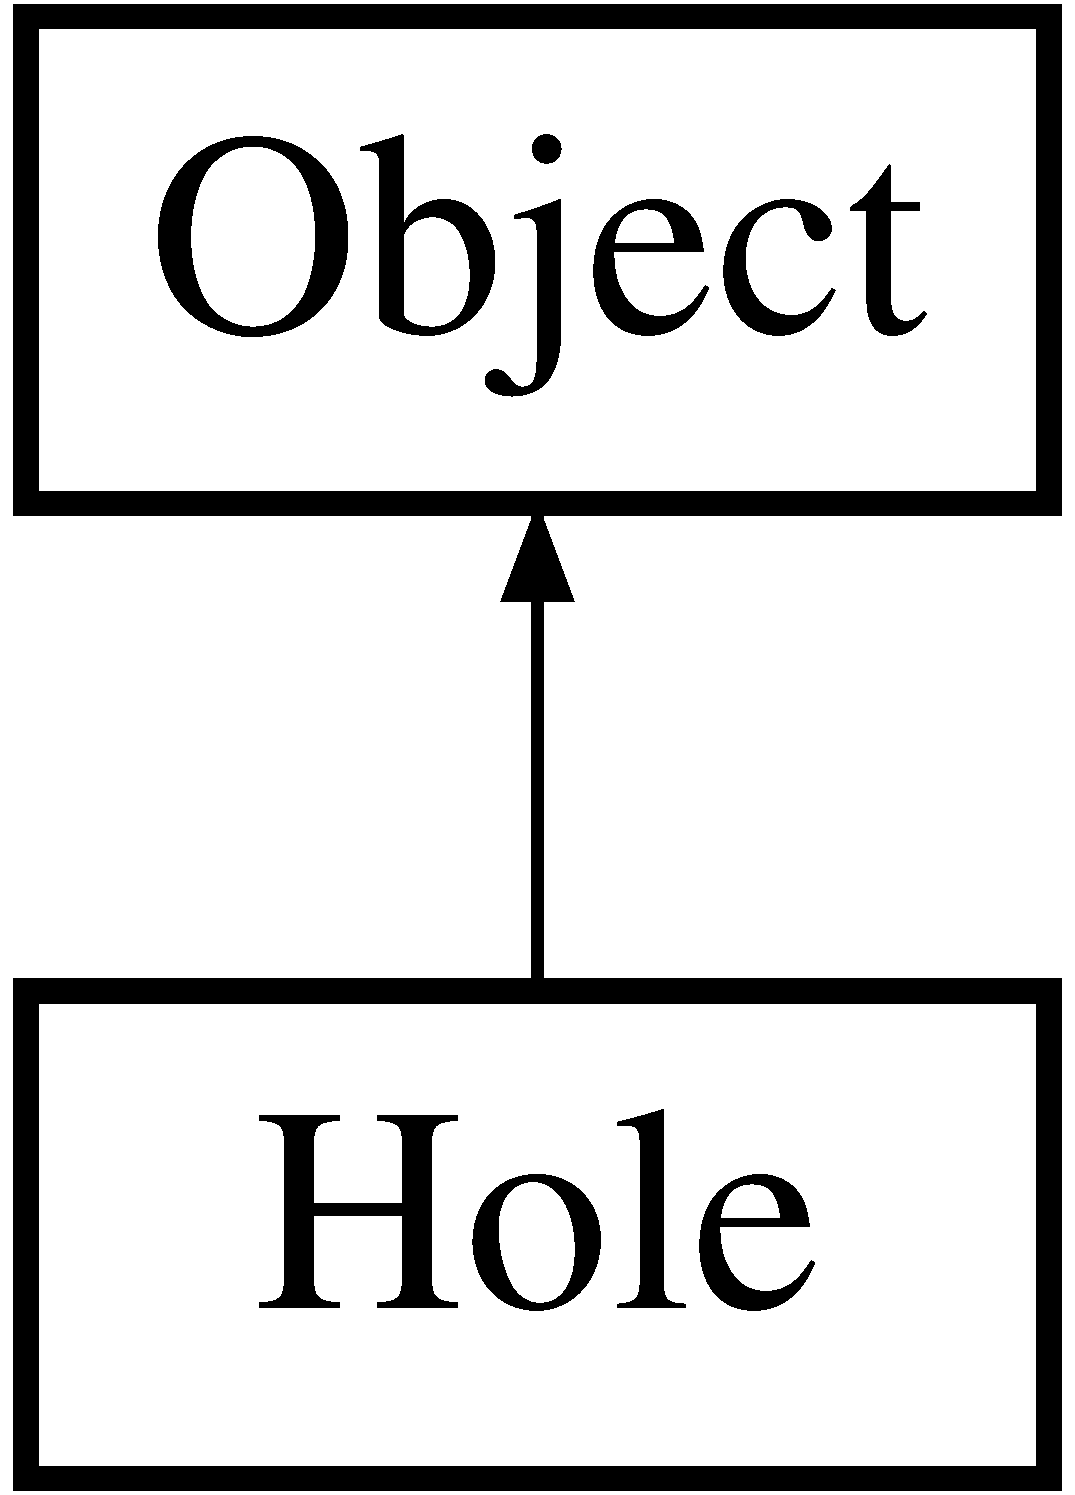
\includegraphics[height=2.000000cm]{class_hole}
\end{center}
\end{figure}
\subsection*{Public Member Functions}
\begin{DoxyCompactItemize}
\item 
\mbox{\Hypertarget{class_hole_a6298a06f04d5f9d91392f4134a0c417e}\label{class_hole_a6298a06f04d5f9d91392f4134a0c417e}} 
bool {\bfseries load\+Avatar} (A\+S\+G\+E\+::\+Renderer $\ast$renderer)
\item 
\mbox{\Hypertarget{class_hole_a553f32907e26768b5fa6eddca0af499f}\label{class_hole_a553f32907e26768b5fa6eddca0af499f}} 
void {\bfseries set\+PosX} (int x) override
\item 
\mbox{\Hypertarget{class_hole_a7d6f0b55d841be9a4d8c37e07e2f2d70}\label{class_hole_a7d6f0b55d841be9a4d8c37e07e2f2d70}} 
void {\bfseries set\+PosY} (int y) override
\end{DoxyCompactItemize}
\subsection*{Additional Inherited Members}


The documentation for this class was generated from the following files\+:\begin{DoxyCompactItemize}
\item 
Projects/\+Snake/Hole.\+h\item 
Projects/\+Snake/Hole.\+cpp\end{DoxyCompactItemize}

\hypertarget{class_object}{}\section{Object Class Reference}
\label{class_object}\index{Object@{Object}}
Inheritance diagram for Object\+:\begin{figure}[H]
\begin{center}
\leavevmode
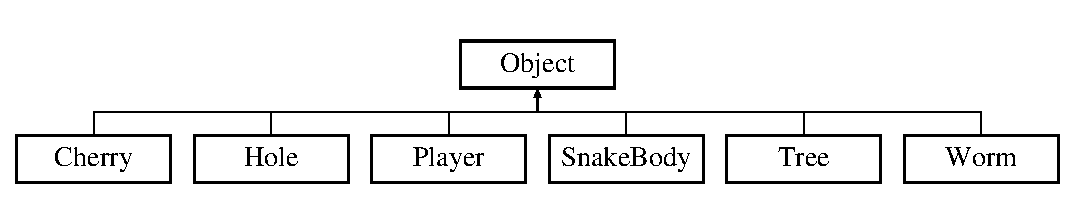
\includegraphics[height=2.000000cm]{class_object}
\end{center}
\end{figure}
\subsection*{Public Member Functions}
\begin{DoxyCompactItemize}
\item 
\mbox{\Hypertarget{class_object_a44005e232ebb49ea093dbf9fb909ef02}\label{class_object_a44005e232ebb49ea093dbf9fb909ef02}} 
virtual bool {\bfseries load\+Avatar} (A\+S\+G\+E\+::\+Renderer $\ast$renderer)=0
\item 
\mbox{\Hypertarget{class_object_a81f5a535d599983bf95089b5e0837c94}\label{class_object_a81f5a535d599983bf95089b5e0837c94}} 
virtual void {\bfseries set\+PosX} (int x)=0
\item 
\mbox{\Hypertarget{class_object_a9684d0c1fd87f92b71423f3615c830db}\label{class_object_a9684d0c1fd87f92b71423f3615c830db}} 
virtual void {\bfseries set\+PosY} (int y)=0
\item 
\mbox{\Hypertarget{class_object_a348ce852463ea723048518d2bd667d09}\label{class_object_a348ce852463ea723048518d2bd667d09}} 
virtual A\+S\+G\+E\+::\+Sprite $\ast$ {\bfseries get\+Object} () const
\item 
\mbox{\Hypertarget{class_object_a7de1555915b05c5d3aac0c2e991c8cd3}\label{class_object_a7de1555915b05c5d3aac0c2e991c8cd3}} 
virtual void {\bfseries get\+Renderer} (A\+S\+G\+E\+::\+Renderer $\ast$renderer)
\item 
\mbox{\Hypertarget{class_object_ae1bd233f42b7fbb51677e7ff570bf999}\label{class_object_ae1bd233f42b7fbb51677e7ff570bf999}} 
virtual int {\bfseries get\+Posx} () const
\item 
\mbox{\Hypertarget{class_object_ac501c5016fc527d03536120d78c1a693}\label{class_object_ac501c5016fc527d03536120d78c1a693}} 
virtual int {\bfseries get\+Posy} () const
\item 
\mbox{\Hypertarget{class_object_a8bd8af22c02e15929c9e5638f2d2bee3}\label{class_object_a8bd8af22c02e15929c9e5638f2d2bee3}} 
virtual void {\bfseries last\+XY} ()
\item 
\mbox{\Hypertarget{class_object_a24a5d4e79c0c7c8599b19ffa68719bc2}\label{class_object_a24a5d4e79c0c7c8599b19ffa68719bc2}} 
virtual int {\bfseries L\+PosX} () const
\item 
\mbox{\Hypertarget{class_object_ac2e2ab5fb648563b3175fc5d338ebe35}\label{class_object_ac2e2ab5fb648563b3175fc5d338ebe35}} 
virtual int {\bfseries L\+PosY} () const
\item 
\mbox{\Hypertarget{class_object_ab6014695762d40c4aed9ddea4c2e024a}\label{class_object_ab6014695762d40c4aed9ddea4c2e024a}} 
virtual void {\bfseries set\+L\+PosX} (int x)
\item 
\mbox{\Hypertarget{class_object_a40d0051b240af9e48743984730f36fb7}\label{class_object_a40d0051b240af9e48743984730f36fb7}} 
virtual void {\bfseries set\+L\+PosY} (int y)
\end{DoxyCompactItemize}
\subsection*{Public Attributes}
\begin{DoxyCompactItemize}
\item 
\mbox{\Hypertarget{class_object_a8ea71e8524ce41f48e9306d057857343}\label{class_object_a8ea71e8524ce41f48e9306d057857343}} 
A\+S\+G\+E\+::\+Sprite $\ast$ {\bfseries avatar} = nullptr
\end{DoxyCompactItemize}
\subsection*{Protected Attributes}
\begin{DoxyCompactItemize}
\item 
\mbox{\Hypertarget{class_object_a7ee7b52ed8eae9689f421ff684bbb047}\label{class_object_a7ee7b52ed8eae9689f421ff684bbb047}} 
int {\bfseries posX}
\item 
\mbox{\Hypertarget{class_object_a022d84d29a80ab6576af10c9e04c8f16}\label{class_object_a022d84d29a80ab6576af10c9e04c8f16}} 
int {\bfseries posY}
\item 
\mbox{\Hypertarget{class_object_abf717e319b3b15409a0bbfc5bec71fbd}\label{class_object_abf717e319b3b15409a0bbfc5bec71fbd}} 
int {\bfseries Last\+Position}
\item 
\mbox{\Hypertarget{class_object_a822da9ea7163e8bbcc258e266858e8bf}\label{class_object_a822da9ea7163e8bbcc258e266858e8bf}} 
int {\bfseries last\+PosX}
\item 
\mbox{\Hypertarget{class_object_a0a8f5d95cd0a6239031519469a03c5d4}\label{class_object_a0a8f5d95cd0a6239031519469a03c5d4}} 
int {\bfseries last\+PosY}
\end{DoxyCompactItemize}


The documentation for this class was generated from the following files\+:\begin{DoxyCompactItemize}
\item 
Projects/\+Snake/Object.\+h\item 
Projects/\+Snake/Object.\+cpp\end{DoxyCompactItemize}

\hypertarget{class_player}{}\section{Player Class Reference}
\label{class_player}\index{Player@{Player}}
Inheritance diagram for Player\+:\begin{figure}[H]
\begin{center}
\leavevmode
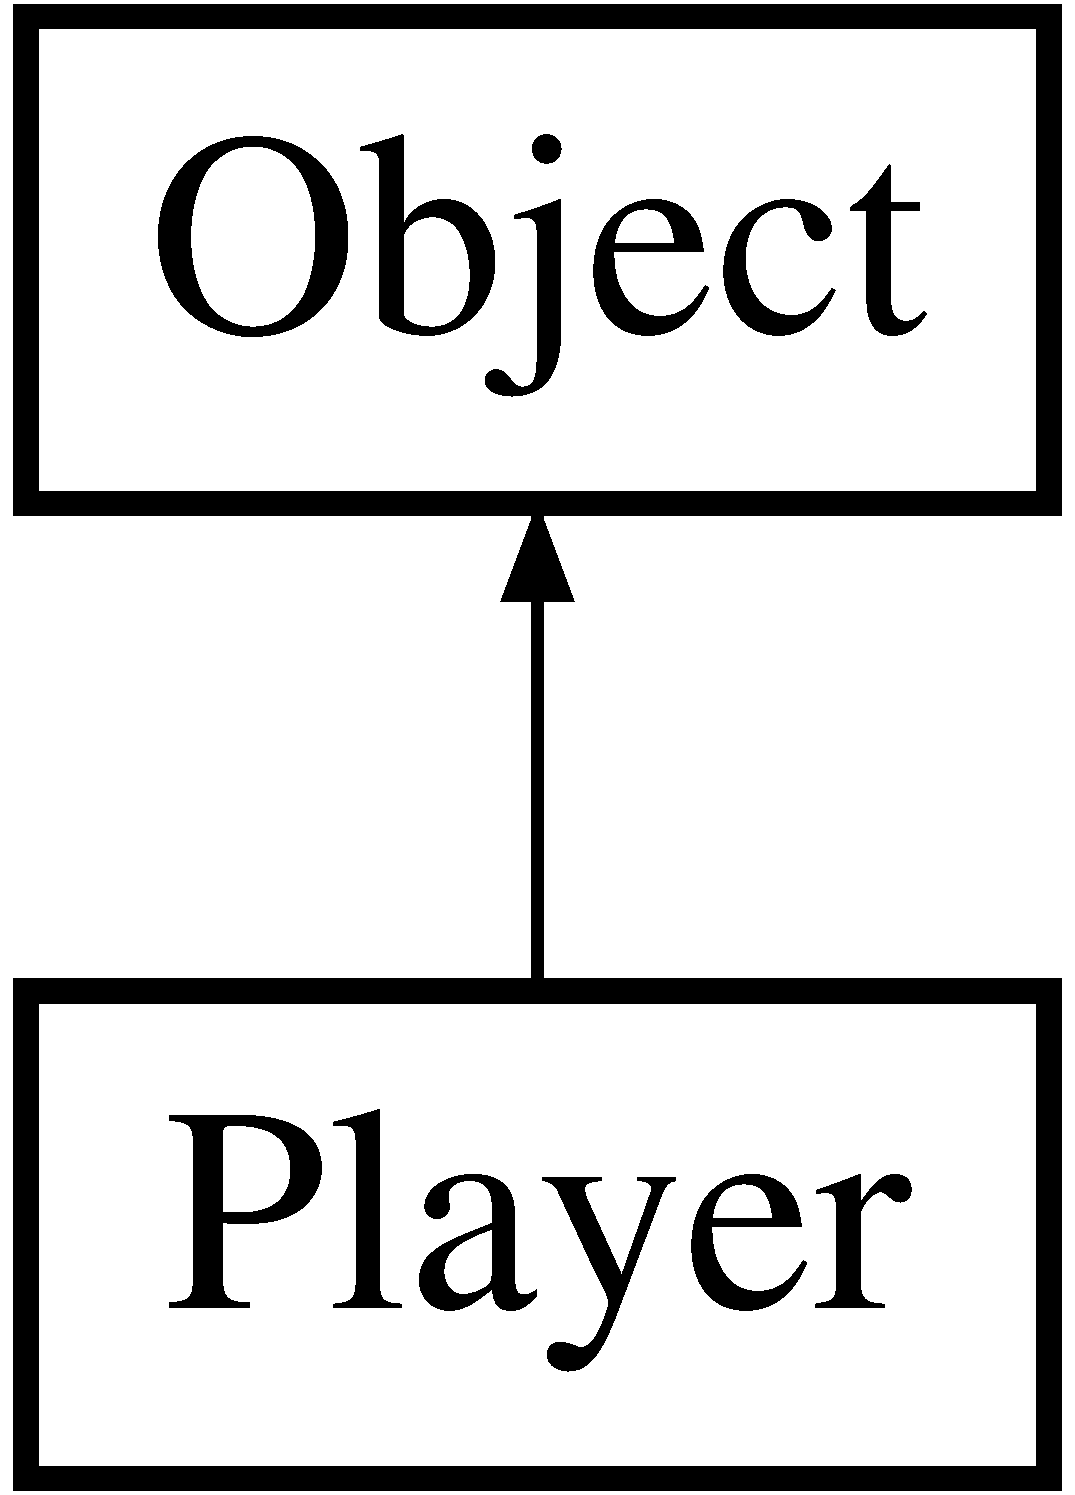
\includegraphics[height=2.000000cm]{class_player}
\end{center}
\end{figure}
\subsection*{Public Member Functions}
\begin{DoxyCompactItemize}
\item 
\mbox{\Hypertarget{class_player_a7ab05ae8247764445129cb8bb217f0cd}\label{class_player_a7ab05ae8247764445129cb8bb217f0cd}} 
bool {\bfseries load\+Avatar} (A\+S\+G\+E\+::\+Renderer $\ast$renderer) override
\item 
\mbox{\Hypertarget{class_player_a88996d2766d3ecc89b8ec55a2ad30430}\label{class_player_a88996d2766d3ecc89b8ec55a2ad30430}} 
void {\bfseries set\+PosX} (int x) override
\item 
\mbox{\Hypertarget{class_player_a3736298c940755ead531cce66213d691}\label{class_player_a3736298c940755ead531cce66213d691}} 
void {\bfseries set\+PosY} (int y) override
\end{DoxyCompactItemize}
\subsection*{Additional Inherited Members}


The documentation for this class was generated from the following files\+:\begin{DoxyCompactItemize}
\item 
Projects/\+Snake/Player.\+h\item 
Projects/\+Snake/Player.\+cpp\end{DoxyCompactItemize}

\hypertarget{class_snake_body}{}\section{Snake\+Body Class Reference}
\label{class_snake_body}\index{Snake\+Body@{Snake\+Body}}
Inheritance diagram for Snake\+Body\+:\begin{figure}[H]
\begin{center}
\leavevmode
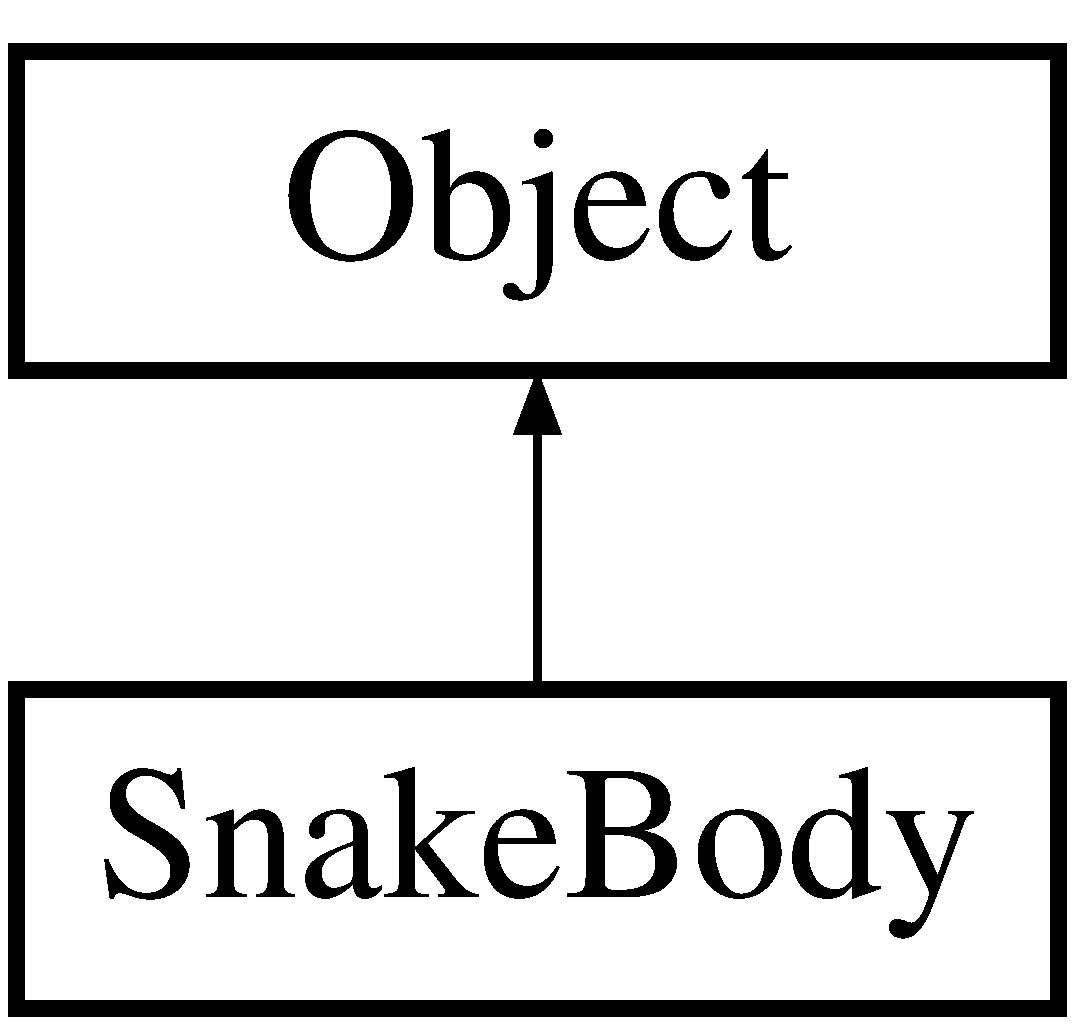
\includegraphics[height=2.000000cm]{class_snake_body}
\end{center}
\end{figure}
\subsection*{Public Member Functions}
\begin{DoxyCompactItemize}
\item 
\mbox{\Hypertarget{class_snake_body_aa2ae5086ef23bed90c1fa79b8099890a}\label{class_snake_body_aa2ae5086ef23bed90c1fa79b8099890a}} 
bool {\bfseries load\+Avatar} (A\+S\+G\+E\+::\+Renderer $\ast$renderer)
\item 
\mbox{\Hypertarget{class_snake_body_aed6b73a5068b8c3c3cee84fdd8361782}\label{class_snake_body_aed6b73a5068b8c3c3cee84fdd8361782}} 
void {\bfseries set\+PosX} (int x) override
\item 
\mbox{\Hypertarget{class_snake_body_adf2a27d12e65237dc7e1e154ad7f32c8}\label{class_snake_body_adf2a27d12e65237dc7e1e154ad7f32c8}} 
void {\bfseries set\+PosY} (int y) override
\end{DoxyCompactItemize}
\subsection*{Additional Inherited Members}


The documentation for this class was generated from the following files\+:\begin{DoxyCompactItemize}
\item 
Projects/\+Snake/Snake\+Body.\+h\item 
Projects/\+Snake/Snake\+Body.\+cpp\end{DoxyCompactItemize}

\hypertarget{class_snake_game}{}\section{Snake\+Game Class Reference}
\label{class_snake_game}\index{Snake\+Game@{Snake\+Game}}


{\ttfamily \#include $<$Game.\+h$>$}

Inheritance diagram for Snake\+Game\+:\begin{figure}[H]
\begin{center}
\leavevmode
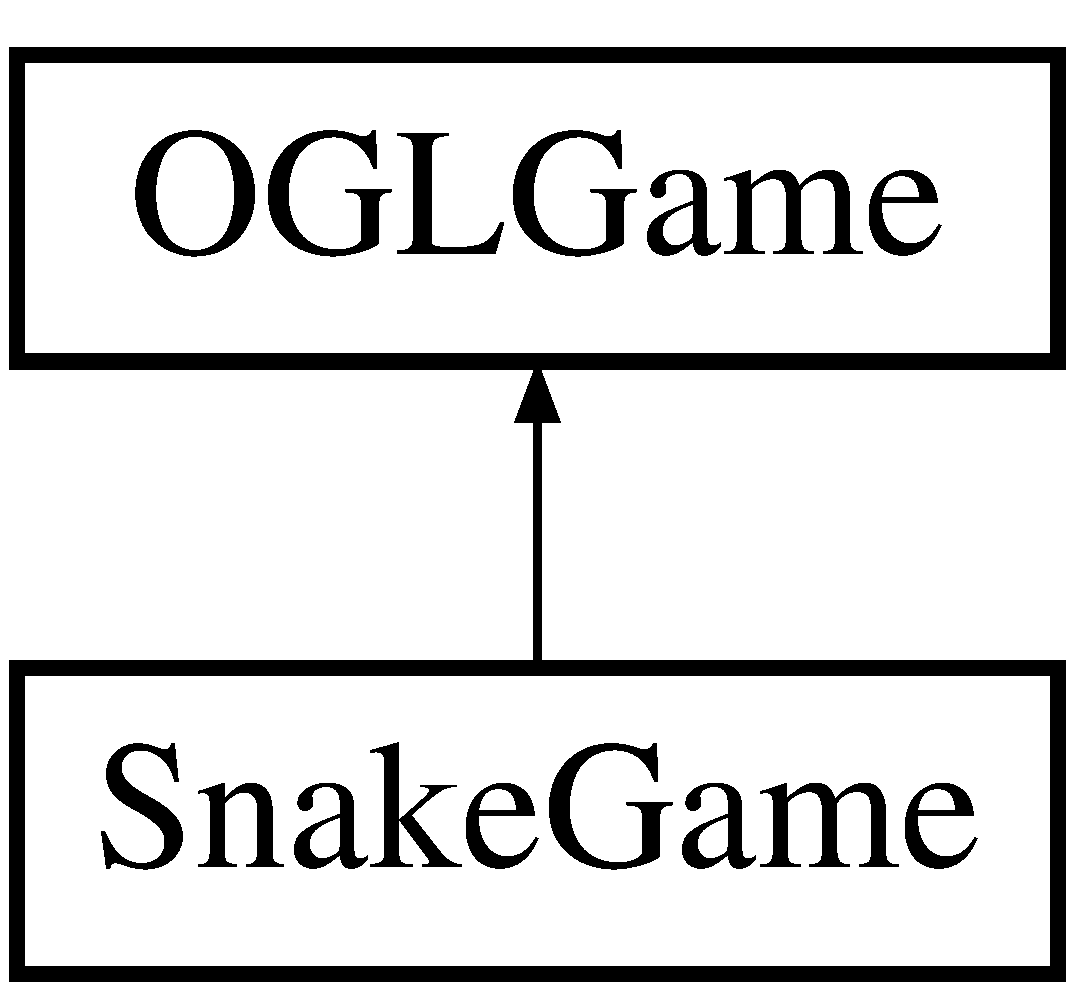
\includegraphics[height=2.000000cm]{class_snake_game}
\end{center}
\end{figure}
\subsection*{Public Member Functions}
\begin{DoxyCompactItemize}
\item 
\hyperlink{class_snake_game_a2a1202d9c2dc3b420e894b7f1581c3a6}{Snake\+Game} ()
\begin{DoxyCompactList}\small\item\em Default Constructor. \end{DoxyCompactList}\item 
virtual bool \hyperlink{class_snake_game_adf792bb503c35e536d905bca53086bbb}{init} () override
\begin{DoxyCompactList}\small\item\em \{ \end{DoxyCompactList}\end{DoxyCompactItemize}
\subsection*{Public Attributes}
\begin{DoxyCompactItemize}
\item 
\mbox{\Hypertarget{class_snake_game_aee5d3cac6bbb0a9b8e6d04fd7d68a7d5}\label{class_snake_game_aee5d3cac6bbb0a9b8e6d04fd7d68a7d5}} 
int {\bfseries tail}
\end{DoxyCompactItemize}


\subsection{Detailed Description}
\hyperlink{class_snake_game}{Snake\+Game}. An Open\+GL Game based on A\+S\+GE. 

\subsection{Constructor \& Destructor Documentation}
\mbox{\Hypertarget{class_snake_game_a2a1202d9c2dc3b420e894b7f1581c3a6}\label{class_snake_game_a2a1202d9c2dc3b420e894b7f1581c3a6}} 
\index{Snake\+Game@{Snake\+Game}!Snake\+Game@{Snake\+Game}}
\index{Snake\+Game@{Snake\+Game}!Snake\+Game@{Snake\+Game}}
\subsubsection{\texorpdfstring{Snake\+Game()}{SnakeGame()}}
{\footnotesize\ttfamily Snake\+Game\+::\+Snake\+Game (\begin{DoxyParamCaption}{ }\end{DoxyParamCaption})}



Default Constructor. 

Destructor.

Remove any non-\/managed memory and callbacks. 

\subsection{Member Function Documentation}
\mbox{\Hypertarget{class_snake_game_adf792bb503c35e536d905bca53086bbb}\label{class_snake_game_adf792bb503c35e536d905bca53086bbb}} 
\index{Snake\+Game@{Snake\+Game}!init@{init}}
\index{init@{init}!Snake\+Game@{Snake\+Game}}
\subsubsection{\texorpdfstring{init()}{init()}}
{\footnotesize\ttfamily bool Snake\+Game\+::init (\begin{DoxyParamCaption}{ }\end{DoxyParamCaption})\hspace{0.3cm}{\ttfamily [override]}, {\ttfamily [virtual]}}



\{ 

Initialises the game.

The game window is created and all assets required to run the game are loaded. The input callback should also be set in the initialise function. \begin{DoxyReturn}{Returns}
True if the game initialised correctly. 
\end{DoxyReturn}


The documentation for this class was generated from the following files\+:\begin{DoxyCompactItemize}
\item 
Source/Game.\+h\item 
Source/Game.\+cpp\end{DoxyCompactItemize}

\hypertarget{class_tree}{}\section{Tree Class Reference}
\label{class_tree}\index{Tree@{Tree}}
Inheritance diagram for Tree\+:\begin{figure}[H]
\begin{center}
\leavevmode
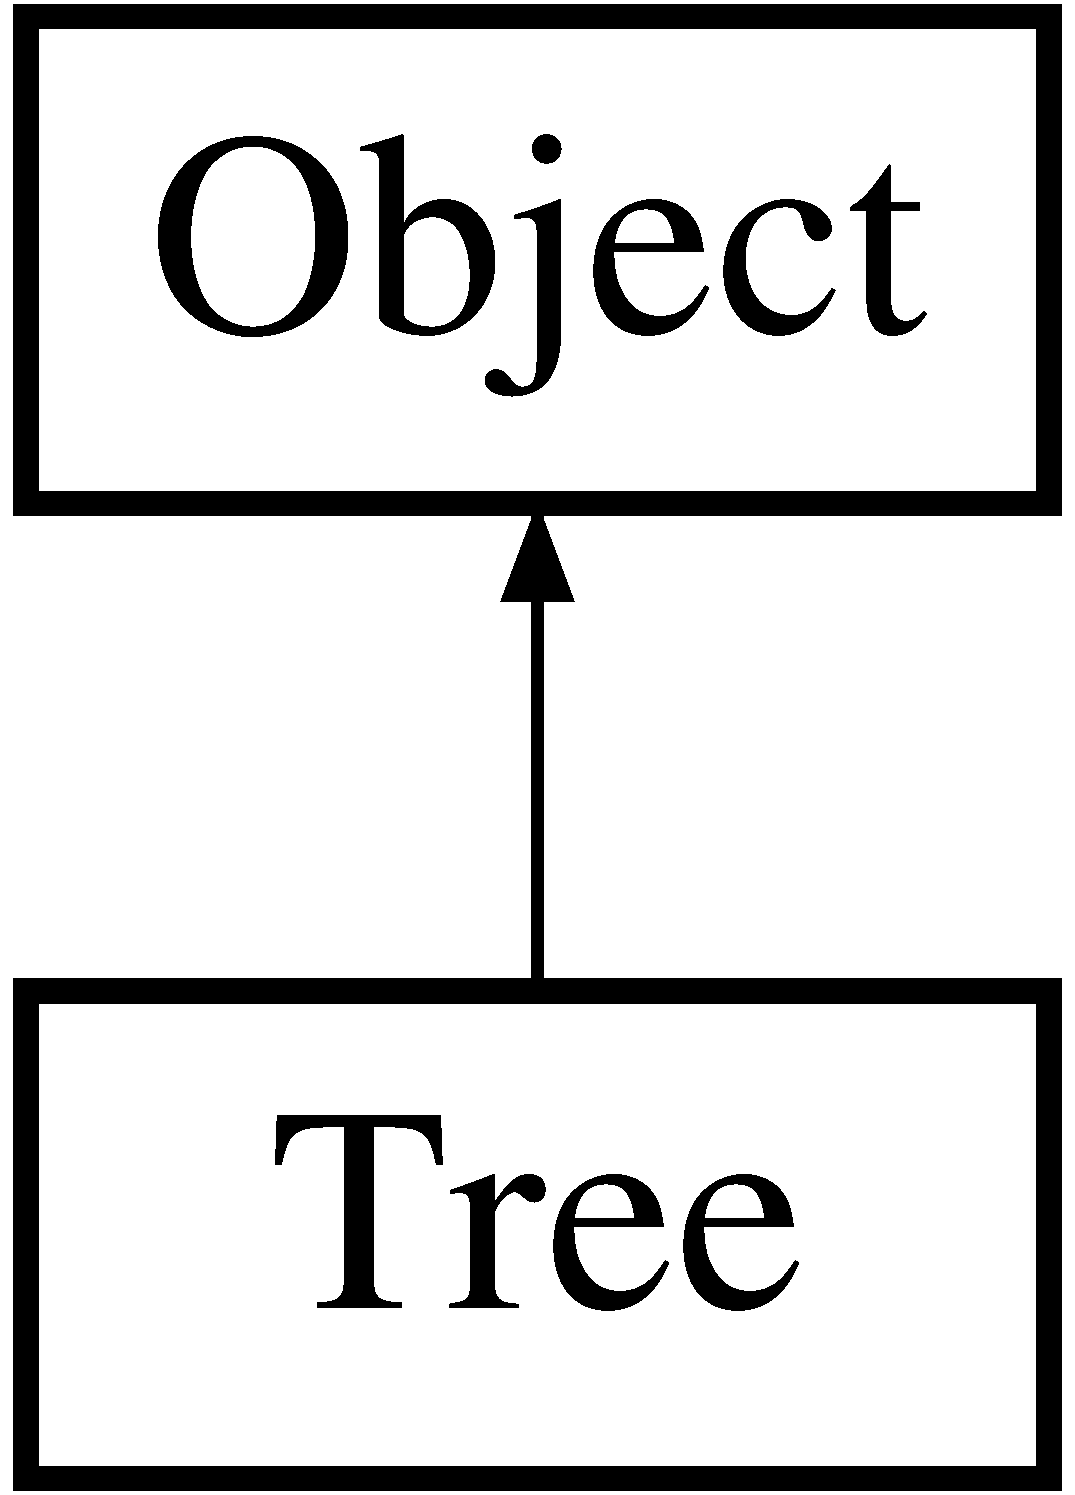
\includegraphics[height=2.000000cm]{class_tree}
\end{center}
\end{figure}
\subsection*{Public Member Functions}
\begin{DoxyCompactItemize}
\item 
\mbox{\Hypertarget{class_tree_add744007ad5d66dabbafa09098712be0}\label{class_tree_add744007ad5d66dabbafa09098712be0}} 
bool {\bfseries load\+Avatar} (A\+S\+G\+E\+::\+Renderer $\ast$renderer) override
\item 
\mbox{\Hypertarget{class_tree_a549c45a5f0414aa7d7ccccfdda572966}\label{class_tree_a549c45a5f0414aa7d7ccccfdda572966}} 
void {\bfseries set\+PosX} (int x) override
\item 
\mbox{\Hypertarget{class_tree_a5a79c7eeabb3785cc6a0d441be0732da}\label{class_tree_a5a79c7eeabb3785cc6a0d441be0732da}} 
void {\bfseries set\+PosY} (int y) override
\end{DoxyCompactItemize}
\subsection*{Additional Inherited Members}


The documentation for this class was generated from the following files\+:\begin{DoxyCompactItemize}
\item 
Projects/\+Snake/Tree.\+h\item 
Projects/\+Snake/Tree.\+cpp\end{DoxyCompactItemize}

\hypertarget{class_worm}{}\section{Worm Class Reference}
\label{class_worm}\index{Worm@{Worm}}
Inheritance diagram for Worm\+:\begin{figure}[H]
\begin{center}
\leavevmode
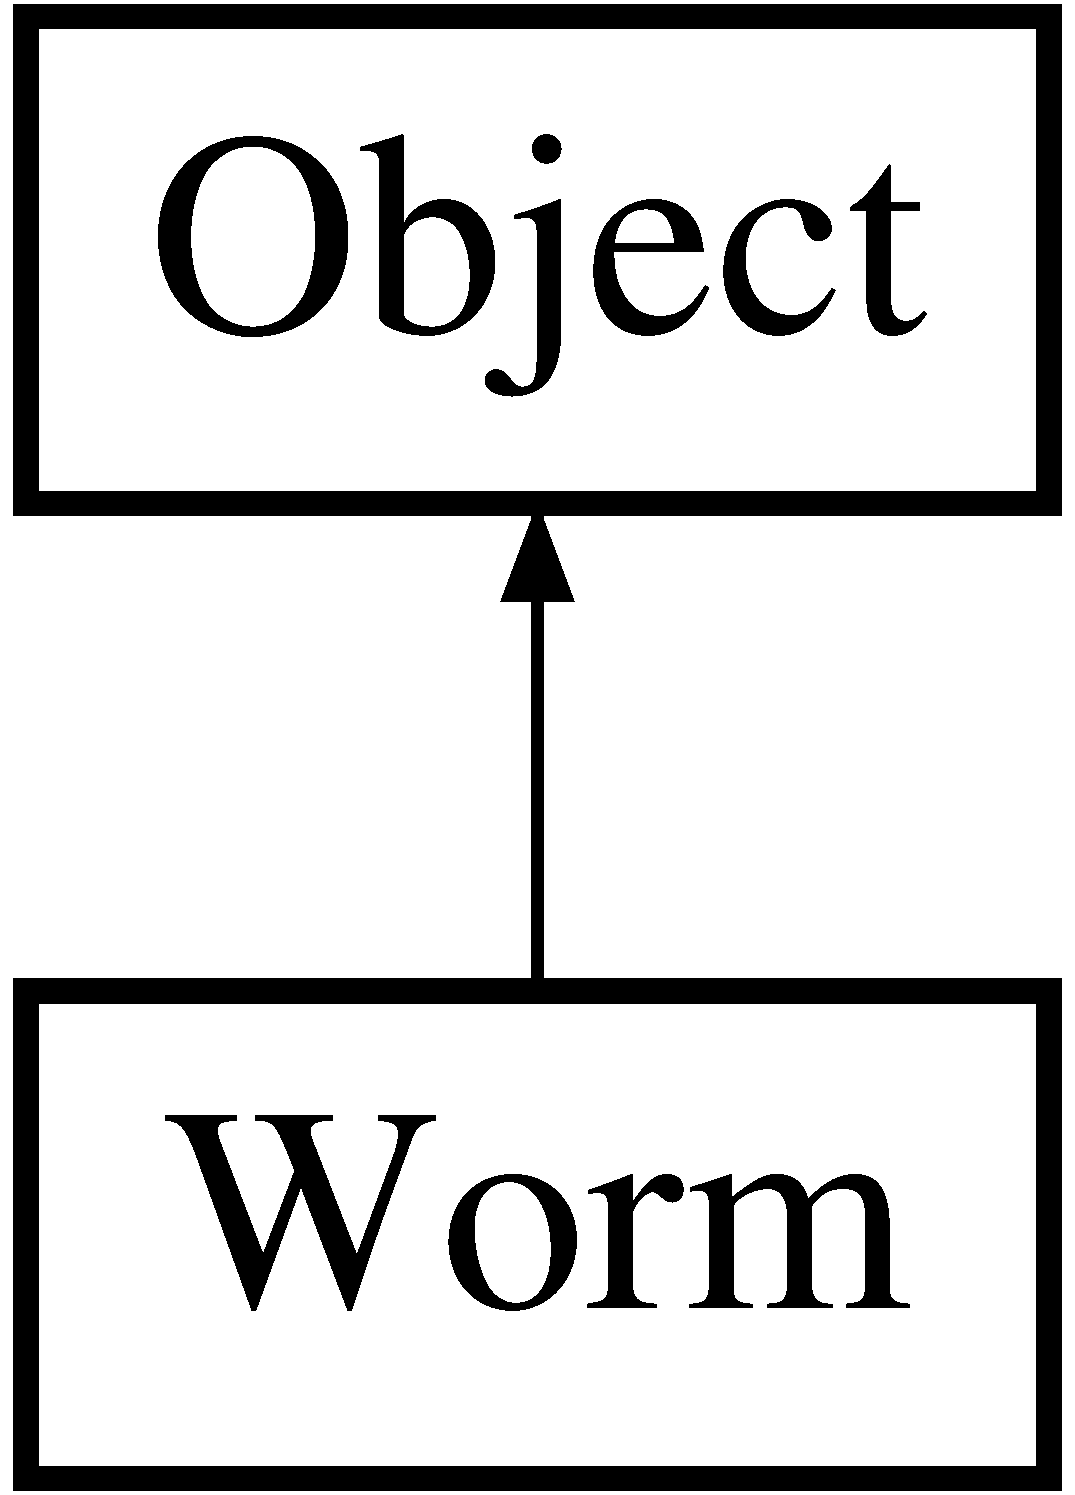
\includegraphics[height=2.000000cm]{class_worm}
\end{center}
\end{figure}
\subsection*{Public Member Functions}
\begin{DoxyCompactItemize}
\item 
\mbox{\Hypertarget{class_worm_ace7384431bf9b69bb12c06b5b563fa0a}\label{class_worm_ace7384431bf9b69bb12c06b5b563fa0a}} 
bool {\bfseries load\+Avatar} (A\+S\+G\+E\+::\+Renderer $\ast$renderer)
\item 
\mbox{\Hypertarget{class_worm_a0b162f66e546cd3a028d33d43386e05f}\label{class_worm_a0b162f66e546cd3a028d33d43386e05f}} 
void {\bfseries set\+PosX} (int x) override
\item 
\mbox{\Hypertarget{class_worm_a543c2f452ff3c6d4567e21a77e4153ca}\label{class_worm_a543c2f452ff3c6d4567e21a77e4153ca}} 
void {\bfseries set\+PosY} (int y) override
\end{DoxyCompactItemize}
\subsection*{Additional Inherited Members}


The documentation for this class was generated from the following files\+:\begin{DoxyCompactItemize}
\item 
Projects/\+Snake/Worm.\+h\item 
Projects/\+Snake/Worm.\+cpp\end{DoxyCompactItemize}

\chapter{File Documentation}
\hypertarget{_actions_8h}{}\section{Source/\+Actions.h File Reference}
\label{_actions_8h}\index{Source/\+Actions.\+h@{Source/\+Actions.\+h}}


The Actions file define a thread safe game action.  


{\ttfamily \#include $<$string$>$}\newline
{\ttfamily \#include $<$atomic$>$}\newline
\subsection*{Enumerations}
\begin{DoxyCompactItemize}
\item 
enum \hyperlink{_actions_8h_a5827805c542ab9cccf700dc3697cbafc}{Game\+Action} \{ \newline
\hyperlink{_actions_8h_a5827805c542ab9cccf700dc3697cbafcaccc0377a8afbf50e7094f5c23a8af223}{Game\+Action\+::\+I\+N\+V\+A\+L\+ID} = -\/1, 
\hyperlink{_actions_8h_a5827805c542ab9cccf700dc3697cbafcab50339a10e1de285ac99d4c3990b8693}{Game\+Action\+::\+N\+O\+NE} = 0, 
{\bfseries E\+X\+IT}, 
\hyperlink{_actions_8h_a5827805c542ab9cccf700dc3697cbafca291554596c183e837f0a6bec3767c891}{Game\+Action\+::\+P\+A\+U\+SE}, 
\newline
{\bfseries S\+T\+A\+RT}, 
{\bfseries G\+A\+M\+E\+O\+V\+ER}, 
{\bfseries H\+O\+LE}
 \}\begin{DoxyCompactList}\small\item\em is a strongly typed enum class representing the next game action \end{DoxyCompactList}
\end{DoxyCompactItemize}
\subsection*{Variables}
\begin{DoxyCompactItemize}
\item 
std\+::atomic$<$ \hyperlink{_actions_8h_a5827805c542ab9cccf700dc3697cbafc}{Game\+Action} $>$ \hyperlink{_actions_8h_a14bdb6dea6cabd733ce612258f33a4b8}{game\+\_\+action}
\end{DoxyCompactItemize}


\subsection{Detailed Description}
The Actions file define a thread safe game action. 

Game\+Actions are stored here as well as a thread safe Game\+Action variable, which has external linkage. 

\subsection{Enumeration Type Documentation}
\mbox{\Hypertarget{_actions_8h_a5827805c542ab9cccf700dc3697cbafc}\label{_actions_8h_a5827805c542ab9cccf700dc3697cbafc}} 
\index{Actions.\+h@{Actions.\+h}!Game\+Action@{Game\+Action}}
\index{Game\+Action@{Game\+Action}!Actions.\+h@{Actions.\+h}}
\subsubsection{\texorpdfstring{Game\+Action}{GameAction}}
{\footnotesize\ttfamily enum \hyperlink{_actions_8h_a5827805c542ab9cccf700dc3697cbafc}{Game\+Action}\hspace{0.3cm}{\ttfamily [strong]}}



is a strongly typed enum class representing the next game action 

\begin{DoxyEnumFields}{Enumerator}
\raisebox{\heightof{T}}[0pt][0pt]{\index{I\+N\+V\+A\+L\+ID@{I\+N\+V\+A\+L\+ID}!Actions.\+h@{Actions.\+h}}\index{Actions.\+h@{Actions.\+h}!I\+N\+V\+A\+L\+ID@{I\+N\+V\+A\+L\+ID}}}\mbox{\Hypertarget{_actions_8h_a5827805c542ab9cccf700dc3697cbafcaccc0377a8afbf50e7094f5c23a8af223}\label{_actions_8h_a5827805c542ab9cccf700dc3697cbafcaccc0377a8afbf50e7094f5c23a8af223}} 
I\+N\+V\+A\+L\+ID&is a non-\/valid game action \\
\hline

\raisebox{\heightof{T}}[0pt][0pt]{\index{N\+O\+NE@{N\+O\+NE}!Actions.\+h@{Actions.\+h}}\index{Actions.\+h@{Actions.\+h}!N\+O\+NE@{N\+O\+NE}}}\mbox{\Hypertarget{_actions_8h_a5827805c542ab9cccf700dc3697cbafcab50339a10e1de285ac99d4c3990b8693}\label{_actions_8h_a5827805c542ab9cccf700dc3697cbafcab50339a10e1de285ac99d4c3990b8693}} 
N\+O\+NE&means no outstanding action to process \\
\hline

\raisebox{\heightof{T}}[0pt][0pt]{\index{P\+A\+U\+SE@{P\+A\+U\+SE}!Actions.\+h@{Actions.\+h}}\index{Actions.\+h@{Actions.\+h}!P\+A\+U\+SE@{P\+A\+U\+SE}}}\mbox{\Hypertarget{_actions_8h_a5827805c542ab9cccf700dc3697cbafca291554596c183e837f0a6bec3767c891}\label{_actions_8h_a5827805c542ab9cccf700dc3697cbafca291554596c183e837f0a6bec3767c891}} 
P\+A\+U\+SE&signals the intention to exit the game \\
\hline

\end{DoxyEnumFields}


\subsection{Variable Documentation}
\mbox{\Hypertarget{_actions_8h_a14bdb6dea6cabd733ce612258f33a4b8}\label{_actions_8h_a14bdb6dea6cabd733ce612258f33a4b8}} 
\index{Actions.\+h@{Actions.\+h}!game\+\_\+action@{game\+\_\+action}}
\index{game\+\_\+action@{game\+\_\+action}!Actions.\+h@{Actions.\+h}}
\subsubsection{\texorpdfstring{game\+\_\+action}{game\_action}}
{\footnotesize\ttfamily std\+::atomic$<$\hyperlink{_actions_8h_a5827805c542ab9cccf700dc3697cbafc}{Game\+Action}$>$ game\+\_\+action}

$<$ Queued Game Action. The next action to be processed as determined by user input. 
\hypertarget{_constants_8h}{}\section{Source/\+Constants.h File Reference}
\label{_constants_8h}\index{Source/\+Constants.\+h@{Source/\+Constants.\+h}}


Constants that are used throughout the game.  


\subsection*{Variables}
\begin{DoxyCompactItemize}
\item 
constexpr int \hyperlink{_constants_8h_a1a4ea27f9b84f4c2a6577f80d51ea998}{W\+I\+N\+D\+O\+W\+\_\+\+W\+I\+D\+TH} = 1600
\item 
constexpr int \hyperlink{_constants_8h_a4653f29f655121ae7b57bc95ef27ad72}{W\+I\+N\+D\+O\+W\+\_\+\+H\+E\+I\+G\+HT} = 1000
\end{DoxyCompactItemize}


\subsection{Detailed Description}
Constants that are used throughout the game. 

Add any new constants to this file. 

\subsection{Variable Documentation}
\mbox{\Hypertarget{_constants_8h_a4653f29f655121ae7b57bc95ef27ad72}\label{_constants_8h_a4653f29f655121ae7b57bc95ef27ad72}} 
\index{Constants.\+h@{Constants.\+h}!W\+I\+N\+D\+O\+W\+\_\+\+H\+E\+I\+G\+HT@{W\+I\+N\+D\+O\+W\+\_\+\+H\+E\+I\+G\+HT}}
\index{W\+I\+N\+D\+O\+W\+\_\+\+H\+E\+I\+G\+HT@{W\+I\+N\+D\+O\+W\+\_\+\+H\+E\+I\+G\+HT}!Constants.\+h@{Constants.\+h}}
\subsubsection{\texorpdfstring{W\+I\+N\+D\+O\+W\+\_\+\+H\+E\+I\+G\+HT}{WINDOW\_HEIGHT}}
{\footnotesize\ttfamily constexpr int W\+I\+N\+D\+O\+W\+\_\+\+H\+E\+I\+G\+HT = 1000}

The window height. Defines the height of the game window \mbox{\Hypertarget{_constants_8h_a1a4ea27f9b84f4c2a6577f80d51ea998}\label{_constants_8h_a1a4ea27f9b84f4c2a6577f80d51ea998}} 
\index{Constants.\+h@{Constants.\+h}!W\+I\+N\+D\+O\+W\+\_\+\+W\+I\+D\+TH@{W\+I\+N\+D\+O\+W\+\_\+\+W\+I\+D\+TH}}
\index{W\+I\+N\+D\+O\+W\+\_\+\+W\+I\+D\+TH@{W\+I\+N\+D\+O\+W\+\_\+\+W\+I\+D\+TH}!Constants.\+h@{Constants.\+h}}
\subsubsection{\texorpdfstring{W\+I\+N\+D\+O\+W\+\_\+\+W\+I\+D\+TH}{WINDOW\_WIDTH}}
{\footnotesize\ttfamily constexpr int W\+I\+N\+D\+O\+W\+\_\+\+W\+I\+D\+TH = 1600}

The window width. Defines how wide the game window is. 
%--- End generated contents ---

% Index
\backmatter
\newpage
\phantomsection
\clearemptydoublepage
\addcontentsline{toc}{chapter}{Index}
\printindex

\end{document}
